\documentclass[16pt,tikz,border=10pt]{standalone}

% Poster typography
\usepackage[T1]{fontenc}
\usepackage{tgheros}
\usepackage[final]{microtype}
\renewcommand{\familydefault}{\sfdefault}

\usepackage{xcolor}
\usepackage{tikz}
\usetikzlibrary{positioning,shadows.blur}

% ---- Palette ----
\definecolor{farsun}{HTML}{1F77B4}   % 2025
\definecolor{plum}{HTML}{9467BD}     % 2026
\definecolor{rob}{HTML}{2CA02C}      % 2026--2027
\definecolor{silso}{HTML}{FF7F0E}    % 2027
\definecolor{slate}{HTML}{1F2937}    % neutral

% ---- Text helpers ----
\newcommand{\CardTitle}[1]{{\bfseries\Large #1}}
\newcommand{\CardText}[1]{{\bfseries\normalsize #1}}

% ---- Global styles ----
\tikzset{
  every node/.style={font=\bfseries, text=slate},
  pinup/.style={densely dashed, line width=1.1pt, draw=#1, opacity=0.95},
  year/.style={text=#1,font=\bfseries\Large},
  cardC/.style 2 args={
    rectangle, rounded corners=3mm, align=left,
    draw=#1!35!black, line width=0.6pt, fill=#1!92,
    text=white, inner sep=7pt, blur shadow,
    text width=#2
  }
}

\begin{document}
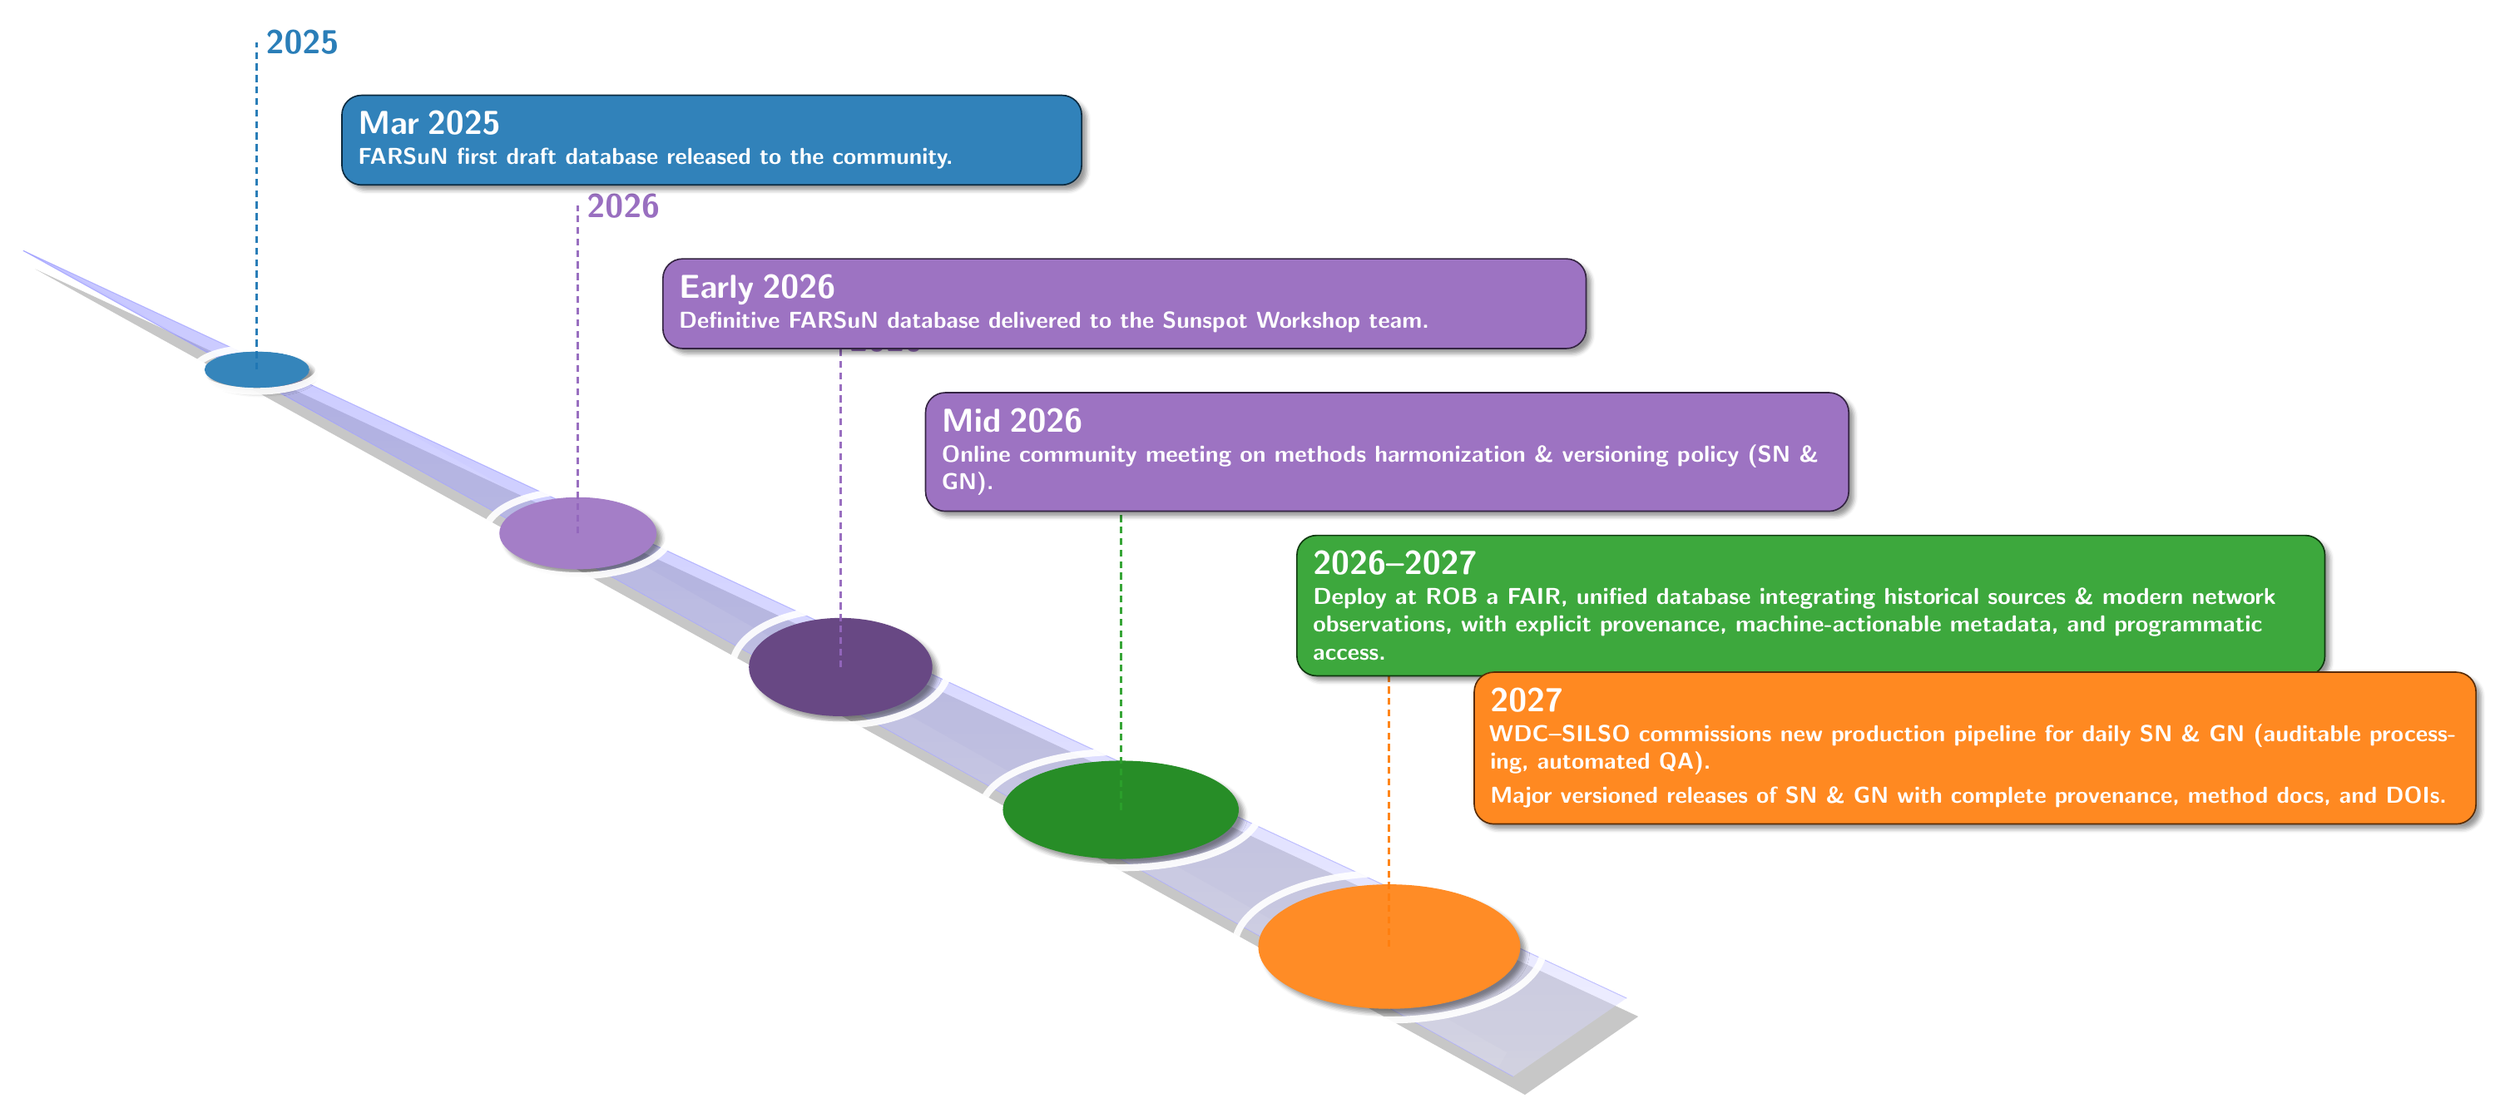
\begin{tikzpicture}[x=1cm,y=1cm]

% =========================
% ROAD (longer, clean, with depth)
% =========================
\def\angUp{-29}
\def\angLo{-25}
\def\lenUp{26.0}     % << longer road
\def\lenLo{27.0}
\coordinate (start) at (-14,1.4);
\coordinate (endA)  at ($(start)+(\angUp:\lenUp)$);
\coordinate (endB)  at ($(start)+(\angLo:\lenLo)$);

% shadow
\begin{scope}[opacity=0.22]
  \fill[black] ($(start)+(0.18,-0.28)$) -- ($(endA)+(0.18,-0.28)$)
               -- ($(endB)+(0.18,-0.28)$) -- cycle;
\end{scope}

% edges
\draw[line join=round,line cap=round,opacity=0.65,
      top color=blue!10,bottom color=blue!60, draw=blue!35]
      (start) -- (endA);
\draw[line join=round,line cap=round,opacity=0.65,
      top color=blue!10,bottom color=blue!60, draw=blue!35]
      (start) -- (endB);

% fill + highlight
\begin{scope}
  \path[clip] (start) -- (endA) -- (endB) -- cycle;
  \shade[bottom color=blue!10, top color=blue!60, opacity=0.45]
        ($(start)+(-1,2)$) rectangle ($(endB)+(1,-2)$);
  \draw[white, line width=12pt, opacity=0.08]
        ($(start)+(0.2,0.18)$) -- ($(endA)+(-0.2,0.18)$);
\end{scope}

% =========================
% MILESTONES (evenly spaced along the road)
% =========================
% distances along road (cm) – feel free to tweak
\def\dA{ 4.0}  % 2025
\def\dB{ 9.5}  % 2026 (delivery)
\def\dC{14.0}  % 2026 (meeting)
\def\dD{18.8}  % 2026–2027 (FAIR DB)
\def\dE{23.4}  % 2027 (ops/releases)

\pgfmathsetmacro{\midang}{(\angUp+\angLo)/2}
\coordinate (P25)  at ($(start)+(\midang:\dA)$);
\coordinate (P26a) at ($(start)+(\midang:\dB)$);
\coordinate (P26b) at ($(start)+(\midang:\dC)$);
\coordinate (P267) at ($(start)+(\midang:\dD)$);
\coordinate (P27)  at ($(start)+(\midang:\dE)$);

% discs + white rims
\foreach \P/\xr/\yr/\clr in {
  P25/8mm/2.8mm/farsun!90,
  P26a/12mm/5.5mm/plum!85,
  P26b/14mm/7.5mm/plum!70!black,
  P267/18mm/7.5mm/rob!88!black,
  P27/20mm/9.5mm/silso!90
}{
  \path[blur shadow, draw=none, fill=\clr] (\P) ellipse [x radius=\xr, y radius=\yr];
  \draw[white, line width=3pt, opacity=0.92] (\P) ellipse [x radius=1.18*\xr, y radius=1.18*\yr];
}

% =========================
% PINS + YEAR LABELS (taller, clear)
% =========================
\def\pinH{5.0} % height of vertical pins
\draw[pinup=farsun] (P25)  -- ++(90:\pinH) node (Y25)  [year=farsun, right] {2025};
\draw[pinup=plum]   (P26a) -- ++(90:\pinH) node (Y26a) [year=plum,   right] {2026};
\draw[pinup=plum]   (P26b) -- ++(90:\pinH) node (Y26b) [year=plum,   right] {2026};
\draw[pinup=rob]    (P267) -- ++(90:\pinH) node (Y267) [year=rob,    right] {2026--2027};
\draw[pinup=silso]  (P27)  -- ++(90:\pinH) node (Y27)  [year=silso,  right] {2027};

% =========================
% RIGHT-SIDE CARDS (just below the year labels; same color; white text)
% =========================
% global offsets from the TOP of each pin
\def\xoff{-0.1} % push right from the label
\def\yoff{-0.8} % place a bit below the year text

% 2025
\node[cardC={farsun}{10.8cm}, anchor=north west]
  at ($(Y25.east)+(\xoff,\yoff)$) {%
  \CardTitle{Mar 2025}\\[1pt]
  \CardText{FARSuN \emph{first draft database} released to the community.}
};

% 2026 (delivery)
\node[cardC={plum}{13.6cm}, anchor=north west]
  at ($(Y26a.east)+(\xoff,\yoff)$) {%
  \CardTitle{Early 2026}\\[1pt]
  \CardText{Definitive FARSuN database delivered to the Sunspot Workshop team.}
};

% 2026 (meeting)
\node[cardC={plum}{13.6cm}, anchor=north west]
  at ($(Y26b.east)+(\xoff,\yoff)$) {%
  \CardTitle{Mid 2026}\\[1pt]
  \CardText{Online community meeting on methods harmonization \& versioning policy (SN \& GN).}
};

% 2026--2027 (FAIR DB)
\node[cardC={rob}{15.2cm}, anchor=north west]
  at ($(Y267.east)+(\xoff,\yoff)$) {%
  \CardTitle{2026--2027}\\[1pt]
  \CardText{Deploy at ROB a FAIR, unified database integrating historical sources \& modern network observations, with explicit provenance, machine-actionable metadata, and programmatic access.}
};

% 2027 (ops + releases)
\node[cardC={silso}{14.8cm}, anchor=north west]
  at ($(Y27.east)+(\xoff,\yoff)$) {%
  \CardTitle{2027}\\[1pt]
  \CardText{WDC--SILSO commissions new production pipeline for daily SN \& GN (auditable processing, automated QA).}\\[3pt]
  \CardText{Major versioned releases of SN \& GN with complete provenance, method docs, and DOIs.}
};

\end{tikzpicture}
\end{document}
